\section{Iterazione 1}

\subsection{Introduzione}
Nella prima iterazione si è scelto di implementare i seguenti casi d'uso:

\begin{itemize}
    \item UC1: Gestione barche \textit{[Astratto]}
          \begin{itemize}
              \item UC1.1 Visualizzazione barche
              \item UC1.2 Inserimento barca
              \item UC1.3 Modifica barca
              \item UC1.4 Eliminazione barca
          \end{itemize}
    \item UC2: Gestione escursioni \textit{[Astratto]}
          \begin{itemize}
              \item UC2.1 Visualizzazione escursioni
              \item UC2.2 Inserimento escursione
              \item UC2.3 Modifica escursione
              \item UC2.4 Eliminazione escursione
          \end{itemize}
    \item UC3: Registrazione utente
    \item UC4: Login utente
    \item UC5: Logout utente
\end{itemize}
In seguito viene riportata una descrizione testuale dei casi d'uso selezionati per la prima iterazione.

\clearpage

\subsection{UC1: Gestione barche}

\emph{Breve descrizione}: il proprietario del diving center deve avere una visione generale e un controllo completo delle sue barche all'interno dell'applicazione.
Oltre alla visualizzazione, il proprietario deve poter modificare ed eliminare le imbarcazioni già presenti nel sistema e poter aggiungerne di nuove.
La gestione delle barche è quindi suddivisa in 4 casi d'uso concreti:

\begin{itemize}
    \item UC1.1 Visualizzazione barche
    \item UC1.2 Inserimento barca
    \item UC1.3 Modifica barca
    \item UC1.4 Eliminazione barca
\end{itemize}

 \emph{Attori coinvolti}: Proprietario, Sistema.\medbreak
 \emph{Trigger}: login del proprietario avvenuto con successo.\medbreak
 \emph{Postcondizione}: il proprietario dopo il login, viene indirizzato alla \textit{owner page} e può scegliere se cliccare uno dei button: \textit{Manage Boat}, \textit{Manage Trip} o \textit{Manage Users}. Cliccando il primo viene indirizzato alla pagina della gestione delle barche (\textit{boat page}), dove vengono visualizzate le barche esistenti ed è presente un tasto \textit{Insert Boat}. \medbreak
 \emph{Procedimento}:

\begin{enumerate}
    \item Proprietario effettua il login.
    \item Sistema mostra la pagina dedicata al proprietario (\textit{owner page}) che comprende 3 bottoni:  \textit{Manage Boat}, \textit{Manage Trip}, \textit{Manage Users}. Cliccando sul primo bottone il proprietario può accedere alla sezione dedicata alla gestione delle barche (\textit{boat page}).
\end{enumerate}

\subsubsection{UC1.1 Visualizzazione barche}

 \emph{Breve descrizione}: Il proprietario visualizza le barche inserite nel sistema e le relative caratteristiche.\medbreak
 \emph{Attori coinvolti}: Proprietario, Sistema.\medbreak
 \emph{Trigger}: Il proprietario clicca il button \textit{Manage Boat}.\medbreak
 \emph{Postcondizione}: Il sistema mostra una vista con l'elenco delle barche.\medbreak
 \emph{Procedimento}:

\begin{enumerate}
    \item Proprietario effettua il login
    \item Proprietario clicca il button \textit{Manage Boat} presente nella owner page.
    \item Sistema mostra l'elenco delle barche presenti nel database con le seguenti informazioni:
          \begin{itemize}
              \item Modello della barca
              \item Capienza della barca
          \end{itemize}
    \item Ogni item dell'elenco è cliccabile. Cliccando su una barca si viene indirizzati ad un'altra pagina che mostra le informazioni della barca e due tasti: \textit{Delete Boat} per eliminare la barca e \textit{Confirm} mediante il quale confermare le eventuali modifiche eseguite sui paramenti della barca. 
\end{enumerate}

\subsubsection{UC1.2 Inserimento barca}

 \emph{Breve descrizione}: Il proprietario aggiunge una barca nel sistema. Questo viene fatto principalmente nella fase iniziale in cui il proprietario deve inserire
tutte le sue barche all'interno dell'applicazione e poi in seguito all'acquisto di nuove barche.\medbreak
 \emph{Attori coinvolti}: Proprietario, Sistema.\medbreak
 \emph{Trigger}: Il proprietario clicca il button \textit{Insert Boat}.\medbreak
 \emph{Postcondizione}: Il sistema mostra la nuova barca all'interno della pagina di visualizzazione delle barche.\medbreak
 \emph{Procedimento}:

\begin{enumerate}
    \item Il proprietario si trova sulla boat page e clicca il button \textit{Insert Boat}.
    \item Il sistema mostra un form in cui è possibile inserire i dati relativi alla barca.
    \item Il proprietario riempie il form.
    \item Il proprietario clicca su \textit{Insert Boat} per inserire la barca nel sistema.
    \item Il sistema mostra la nuova barca all'interno della pagina di visualizzazione delle barche \textit{boat page}.
\end{enumerate}

\subsubsection{UC1.3 Modifica barca}

 \emph{Breve descrizione}: Il proprietario si trova sulla pagina di visualizzazione delle barche. Cliccando su una barca viene visualizzata la pagina relativa alle informazioni della barca selezionata. In questa pagina il proprietario può modificare le informazioni della barca e poi cliccare il tasto  \textit{Confirm} per confermare. 

\medbreak
 \emph{Attori coinvolti}: Proprietario, Sistema.\medbreak
 \emph{Trigger}: Il proprietario clicca sulla barca che vuole modificare.\medbreak
 \emph{Postcondizione}: Il sistema mostra la barca modificata all'interno della pagina di visualizzazione delle barche \textit{boat page}.\medbreak
 \emph{Procedimento}:

\begin{enumerate}
    \item Il proprietario si trova sulla pagina di visualizzazione delle barche (\textit{boat page}) e clicca su una specifica barca.
    \item Il sistema mostra una vista in cui è possibile modificare i dati relativi alla barca.
    \item Il proprietario modifica i dati.
    \item Il proprietario clicca su \textit{Confirm} per confermare le modifiche dei dati della barca.
    \item Il sistema mostra la barca aggiornata all'interno della pagina di visualizzazione delle barche.
\end{enumerate}

\subsubsection{UC1.4 Eliminazione barca}

 \emph{Breve descrizione}: Il proprietario si trova sulla pagina di visualizzazione delle barche e clicca su una barca, accede alla pagina relativa alle informazioni della barca selezionata. In questa pagina il proprietario sceglie di eliminare la barca cliccando sul bottone \textit{Delete}. 
L'eliminazione può essere definitiva o temporanea. L'eliminazione è definitiva se la barca non è più agibile o perché viene sostituita da un'altra;
è temporanea nel caso in cui sia necessaria attività di manutenzione.\medbreak
 \emph{Attori coinvolti}: Proprietario, Sistema.\medbreak
 \emph{Trigger}: Il proprietario clicca sulla barca da eliminare.\medbreak
 \emph{Postcondizione}: Il sistema mostra la pagina di visualizzazione delle barche in cui non comparirà la barca eliminata.\medbreak
 \emph{Procedimento}:

\begin{enumerate}
    \item Il proprietario si trova sulla pagina di visualizzazione delle barche (\textit{boat page}) e clicca su una barca specifica. 
    \item Il sistema mostra una pagina con le informazioni relative a quella barca e i bottoni \textit{Confirm} e \textit{Delete}.
    \item Il proprietario clicca sul tasto \textit{Delete}.
    \item Il sistema mostra la pagina di visualizzazione delle barche in cui non comparirà la barca eliminata.
\end{enumerate}

\clearpage

\subsection{UC2: Gestione escursioni}
L'applicazione deve poter semplificare la gestione e l'organizzazione delle escursioni al proprietario del diving center.
L'applicazione deve fungere da calendario, mettendo a disposizione le seguenti funzionalità:

\begin{itemize}
    \item UC2.1 Visualizzazione escursioni
    \item UC2.2 Inserimento escursione
    \item UC2.3 Modifica escursione
    \item UC2.4 Eliminazione escursione
\end{itemize}

\subsubsection{UC2.1 Visualizzazione escursioni}

 \emph{Breve descrizione}: Il proprietario visualizza le date e i turni in cui gli utenti possono prenotarsi.\medbreak
 \emph{Attori coinvolti}: Proprietario, Sistema.\medbreak
 \emph{Trigger}: Il proprietario clicca il button \textit{Manage Trip}.\medbreak
 \emph{Postcondizione}: Il sistema mostra una vista con l'elenco delle escursioni.\medbreak
 \emph{Procedimento}:

\begin{enumerate}
    \item Il proprietario effettua il login.
    \item Il sistema mostra la pagina dedicata al proprietario (\textit{owner page}) che comprende 3 bottoni:  \textit{Manage Boat}, \textit{Manage Trip}, \textit{Manage Users}. Cliccando sul bottone  \textit{Manage Trip} il proprietario può accedere alla sezione dedicata alla gestione delle escursioni (\textit{trip page}).
    \item Il proprietario clicca il button \textit{Manage Trip} presente nella \textit{owner page}.
    \item Il sistema mostra la \textit{trip page} contenente l'elenco delle escursioni e un bottone \textit{Insert trip}. 
    Ogni escursione viene visualizzata con le seguenti informazioni:
          \begin{itemize}
              \item Data.
              \item Orario di inizio.
          \end{itemize}
    \item Ogni escursione presente nell'elenco è cliccabile. Cliccando su un'escursione si viene indirizzati ad un'altra pagina, in cui vengono mostrate le informazioni dell'escursione. Inoltre sono presenti due tasti: \textit{Delete} per eliminare l'escursione e \textit{Confirm} per confermare eventuali modifiche apportate alle informazioni relative all'escursione.   
\end{enumerate}

\subsubsection{UC2.2 Inserimento escursione}

 \emph{Breve descrizione}: Il proprietario aggiunge un'escursione al calendario indicandone data e orario in cui verranno rese disponibili le prenotazioni.\medbreak
 \emph{Attori coinvolti}: Proprietario, Sistema.\medbreak
 \emph{Trigger}: Il proprietario clicca il button \textit{Insert trip}.\medbreak
 \emph{Postcondizione}: Il sistema mostra la nuova escursione all'interno della pagina di visualizzazione delle escursioni.\medbreak
 \emph{Procedimento}:

\begin{enumerate}
    \item Il proprietario si trova sulla \textit{trip page} e clicca il bottone \textit{Insert trip}.
    \item Il sistema mostra un form in cui è possibile inserire i dati relativi all'escursione.
    \item Il proprietario riempie il form.
    \item Il proprietario clicca su \textit{Confirm} per inserire l'escursione nel sistema.
    \item Il sistema mostra la nuova escursione all'interno della pagina di visualizzazione delle escursioni \textit{trip page}.
\end{enumerate}

\subsubsection{UC2.3 Modifica escursione}

 \emph{Breve descrizione}: Il proprietario si trova sulla pagina di visualizzazione delle escursioni, clicca su una specifica escursione e viene indirizzato ad una nuova pagina che mostra le informazioni dell'escursione selezionata. Nella pagina sono presenti anche due bottoni: \textit{Confirm} e \textit{Delete}.
Tale modifica può essere dovuta a cambiamenti climatici o ad altri imprevisti.\medbreak
 \emph{Attori coinvolti}: Proprietario, Sistema.\medbreak
 \emph{Trigger}: Il proprietario clicca su un'escursione.\medbreak
 \emph{Postcondizione}: Il sistema mostra l'escursione modificata all'interno della pagina di visualizzazione delle escursioni.\medbreak
 \emph{Procedimento}:

\begin{enumerate}
    \item Il proprietario si trova sulla pagina di visualizzazione delle escursioni e clicca su un'escursione.
    \item Sistema mostra una vista in cui è possibile modificare i dati relativi all'escursione.
    \item Proprietario modifica i dati.
    \item Proprietario clicca su \textit{Confirm} per modificare i dati dell'escursione.
    \item Il sistema mostra l'escursione aggiornata all'interno della pagina di visualizzazione delle escursioni.
\end{enumerate}

\subsubsection{UC2.4 Eliminazione escursione}

 \emph{Breve descrizione}: Il proprietario si trova sulla pagina di visualizzazione delle escursioni, clicca su un'escursione e viene indirizzato ad una nuova pagina che mostra le informazioni dell'escursione selezionata. Nella pagina sono presenti anche i bottoni \textit{Confirm} e \textit{Delete}.\medbreak
 \emph{Attori coinvolti}: Proprietario, Sistema.\medbreak
 \emph{Trigger}: Il proprietario clicca il bottone \textit{Delete}.\medbreak
 \emph{Postcondizione}: Il sistema mostra la pagina di visualizzazione delle escursioni in cui non comparirà l'escursione eliminata.\medbreak
 \emph{Procedimento}:

\begin{enumerate}
    \item Il proprietario si trova sulla pagina di visualizzazione delle escursioni e clicca su un'escursione.
    \item Il sistema mostra la pagina relativa all'escursione selezionata, contenente anche i bottoni \textit{Confirm} e \textit{Delete}.
    \item Il proprietario clicca il bottone \textit{Delete}.
    \item Il sistema mostra la pagina di visualizzazione delle escursioni in cui non comparirà l'escursione eliminata.
\end{enumerate}

\clearpage

\subsection{UC3: Registrazione dell'utente}
 \emph{Breve descrizione}: L'utente compila il form per la registrazione al servizio e viene aggiunto al database. La registrazione non può avvenire per utenti già registrati.\medbreak
 \emph{Attori coinvolti}: Utente, Sistema.\medbreak
 \emph{Trigger}: L'utente preme il bottone \textit{Registrazione}.\medbreak
 \emph{Postcondizione}: L'utente è stato inserito nel database e ha ricevuto la conferma dell'operazione.\medbreak
 \emph{Procedimento}:
\begin{enumerate}
    \item L'utente preme il bottone \textit{Registrazione} nella \textit{Homepage}.
    \item L'utente fornisce le seguenti informazioni nel form di registrazione:
    \begin{itemize}
        \item Nome
        \item Cognome
        \item Email
        \item Password
        \item Numero di brevetto
    \end{itemize}
    \item Il sistema verifica se l'email inserita è già associata ad un altro utente registrato:
          \begin{enumerate}
              \item se l'email esiste, il sistema impedisce la registrazione e lo comunica all'utente
              \item se l'email non esiste, il sistema aggiunge l'utente nel database.
          \end{enumerate}
\end{enumerate}

\clearpage
\subsection{UC4: Login dell'utente}
 \emph{Breve descrizione}: L'utente o il proprietario compila il form per il login; in caso di credenziali corrette il sistema consente l'accesso al servizio.\medbreak
 \emph{Attori coinvolti}: Utente/Proprietario, Sistema.\medbreak
 \emph{Trigger}: L'utente preme sul bottone \textit{Login}. \medbreak
 \emph{Postcondizione}: Nel caso l'utente sia un amministratore verrà indirizzato alla \textit{owner page}, altrimenti alla \textit{user page}. \medbreak
 \emph{Procedimento}:
\begin{enumerate}
    \item L'utente preme su \textit{Login} nella pagina iniziale dell'app
    \item L'utente fornisce username e password nel form di registrazione
    \item Il sistema controlla le credenziali inserite:
          \begin{enumerate}
              \item se sono corrette, avviene il login e il sistema invia una conferma di accesso all'utente
              \item se sono errate, viene impedito il login e notificato il mancato accesso all'utente.
          \end{enumerate}
\end{enumerate}

\subsection{UC5: Logout dell'utente}
 \emph{Breve descrizione}: Il sistema effettua il logout dell'utente dall'applicazione.\medbreak
 \emph{Attori coinvolti}: Utente, Sistema.\medbreak
 \emph{Trigger}: L'utente preme il tasto \textit{back button} della \textit{owner page} o della \textit{user page} e viene reindirizzato alla \textit{Homepage}. In questa pagina è presente la sezione per effettuare il \textit{Login} o la \textit{Registrazione}.  \medbreak
 \emph{Postcondizione}: Il sistema mostra la \textit{Homepage}. \medbreak
 \emph{Procedimento}:
\begin{enumerate}
    \item L'utente preme il \textit{back button} della \textit{owner page} o  della \textit{user page}
    \item Il sistema effettua il logout dell'utente e mostra la \textit{Homepage}. 
\end{enumerate}

\subsection{UML Component Diagram}
Partendo dai casi d'uso selezionati per questa iterazione e procedendo con l'utilizzo delle euristiche di design, è stato possibile progettare l'architettura software del nostro sistema. I casi d'uso sono stati raggruppati in base all'affinità e per ognuno è stato introdotto un componente \textit{boundary}, un componente \textit{control} e un componente \textit{data}. 

\begin{itemize}
    \item <<boundary>> componenti lato front-end con cui gli attori si interfacciano direttamente. 
    \item <<control>>  componenti lato back-end che gestiscono la logica del programma e espongono delle API al front-end, richiedendone a loro volta al database.
    \item <<data>> componenti lato back-end che interagiscono con il database.
\end{itemize}

\begin{figure}[htbp]
    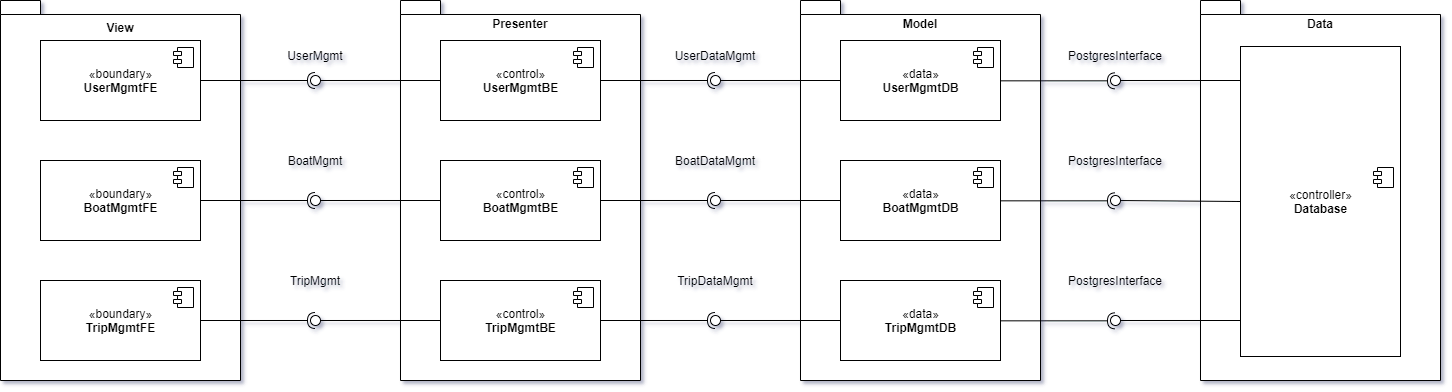
\includegraphics[width=\textwidth]{iterazione1/diagrams/ComponentDiagram_v4.png}
    \centering
    \caption{UML Component Diagram}\label{fig:componentDiagram}
\end{figure}

\newpage

\subsection{UML Class Diagram per interfacce}
Il diagramma in Figura~\ref{fig:ClassDiagramInterfaces} mostra le interfacce del sistema con le relative funzioni e i dati di input e output. Il diagramma evidenzia anche i layers del design pattern Model View Presenter.

\begin{figure}[htbp]
    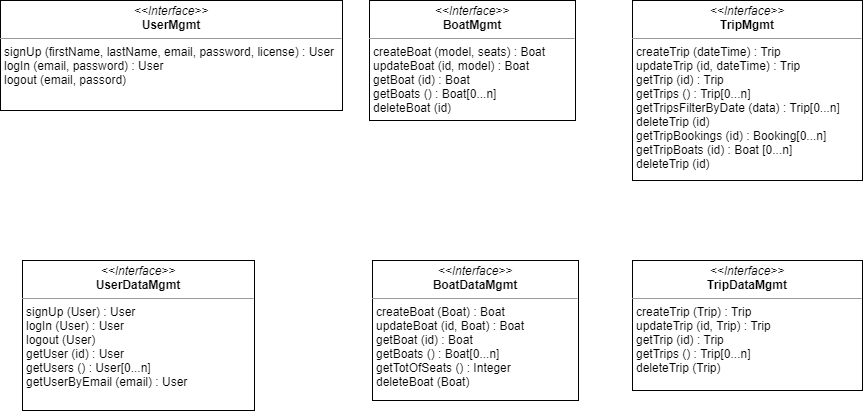
\includegraphics[width=\textwidth]{iterazione1/diagrams/ClassDiagramInterfaces_v6.png}
    \centering
    \caption{UML Class Diagram per interfacce}
    \label{fig:ClassDiagramInterfaces}
\end{figure}

\newpage

\subsection{UML Class Diagram per tipi di dato}
Il diagramma in Figura~\ref{fig:ClassDiagramTypes} mostra i tipi di dato necessari allo sviluppo dell'applicazione. Per la progettazione dei tipi di dato e delle interfacce sono state seguite le euristiche di design. 

\begin{figure}[htbp]
    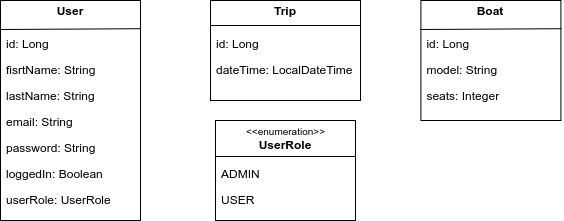
\includegraphics[width=\textwidth]{iterazione1/diagrams/ClassDiagramTypes_v3.png}
    \centering
    \caption{UML Class Diagram per tipi di dato}
    \label{fig:ClassDiagramTypes}
\end{figure}

\clearpage
\subsection{UML Deployment Diagram}
Mediante l'utilizzo di un Deployment Diagram UML è possibile mostrare la rappresentazione hardware e software del sistema. In Figura~\ref{fig:DeploymentDiagram} vengono mostrati i componenti contenuti nei seguenti nodi:

\begin{itemize}
    \item Cellulare proprietario, nodo su cui l'admin del sistema potrà gestire le barche e il calendario delle escursioni.
    \item Cellulare utente, nodo su cui un soggetto potrà registrarsi alla piattaforma.
    \item Web Server, espone le API richieste lato front-end.
    \item Database, funge da storage dei dati.
\end{itemize}

\begin{figure}[htbp]
    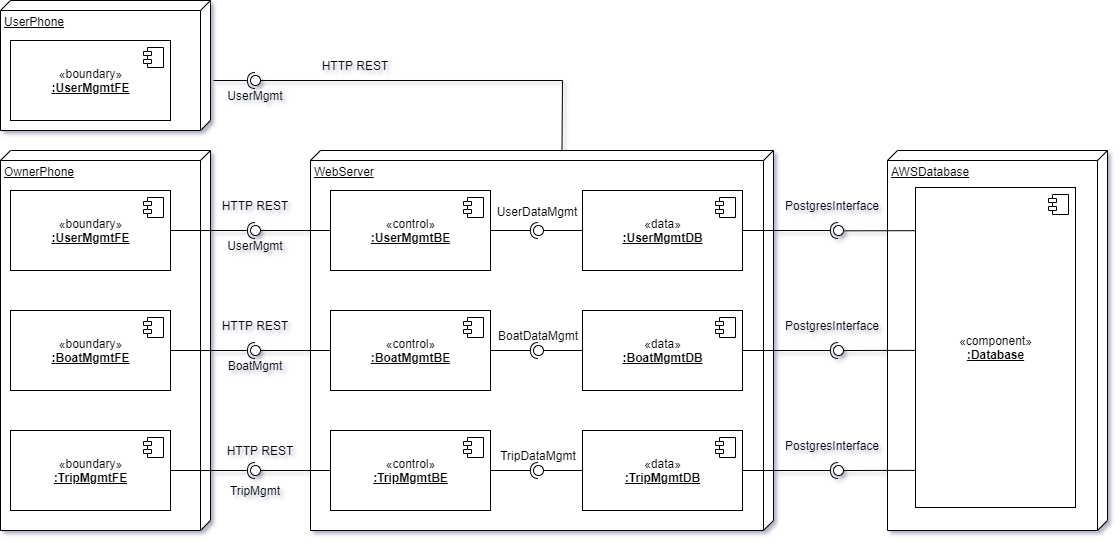
\includegraphics[width=\textwidth]{iterazione1/diagrams/DeploymentDiagram_v6.png}
    \centering
    \caption{UML Deployment Diagram}
    \label{fig:DeploymentDiagram}
\end{figure}

\clearpage

\subsection{Testing}

\subsubsection{Analisi statica}
Come visto nel paragrafo \ref{analisi-statica} è stata utilizzata l'estensione \textit{Language Support for Java(TM) by Red Hat} fornita
dall'IDE \textit{Visual Studio Code}.

\subsubsection{Analisi dinamica}
Per l'iterazione 1 è stato effettuato il test delle seguenti funzioni:
\begin{itemize}
  \item Login con credenziali corrette
  \item Login con credenziali errate
  \item Logout a buon fine
  \item Creazione barca a buon fine
  \item Visualizzazione escursioni filtrate per data a buon fine
\end{itemize}

I risultati sono riportati in Figura \ref{Risultati test dinamico iterazione 1}. 

\begin{figure}[htbp]
    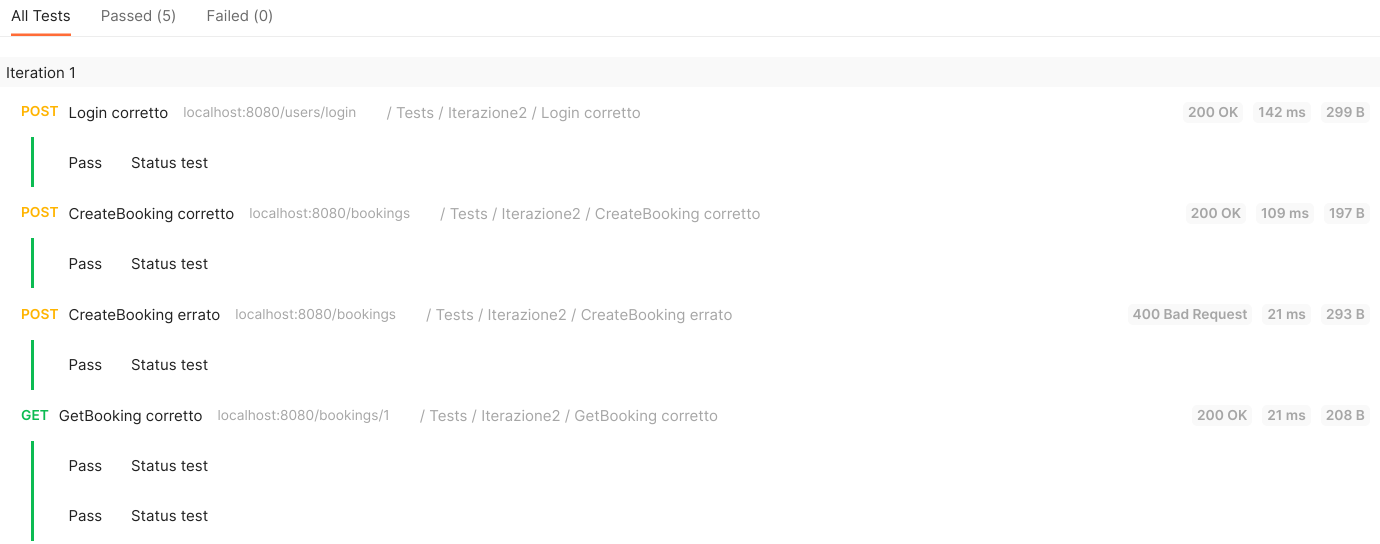
\includegraphics[width=\textwidth]{iterazione1/test/service-test.png}
    \centering
    \caption{Risultati test dinamico}
    \label{Risultati test dinamico iterazione 1}
\end{figure}
\subsubsection{Unit Test}
Per questa iterazione è stata testata la funzione \textit{findByDateTime} presente nel back-end, che serve a filtrare le escursioni e ottenere solo quelle relative ad una certa data.

\begin{lstlisting}[language=Java]
@DataJpaTest
class TripRepositoryTest {

    @Autowired
    private TripRepository underTest;

    @Test
    void findByDateTime() {
        // given
        LocalDateTime date = LocalDateTime.of
        (2022, Month.JANUARY, 01, 10, 00, 00);
        Trip expected = new Trip(date);
        underTest.save(expected);

        // when
        Trip result = underTest.findByDateTime(date).get(0);

        // then
        assertThat(expected).isEqualTo(result);
    }
}
\end{lstlisting}

Il test di unità con JUnit ha confermato la correttezza della funzione. 

\begin{figure}[htbp]
    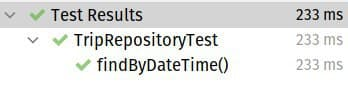
\includegraphics[width=\textwidth]{images/iterazione1/test/unit-test.jpg}
    \centering
    \caption{Risultato Unit Test}
    \label{test jUnit findByDateTime}
\end{figure}

\subsection{Documentazione API}
In questa sezione vengono mostrate alcune delle API sviluppate per l'iterazione 1. È possibile visualizzare tutte le API mediante la collezione di Postman che è possibile scaricare dalla repository su GitHub.  
\begin{itemize}
    \item API per la creazione di una barca. Figura \ref{creazione barca}
    \item API per la creazione di un'escursione. Figura \ref{creazione escursione}
    \item API per la visualizzazione di escursioni relative ad un giorno specifico. Figura \ref{trip} 
    \item API per il Login di un utente. Figura \ref{login}
    \item API per la registrazione di un utente. Figura \ref{signup}
\end{itemize}

\begin{figure}[htbp]
    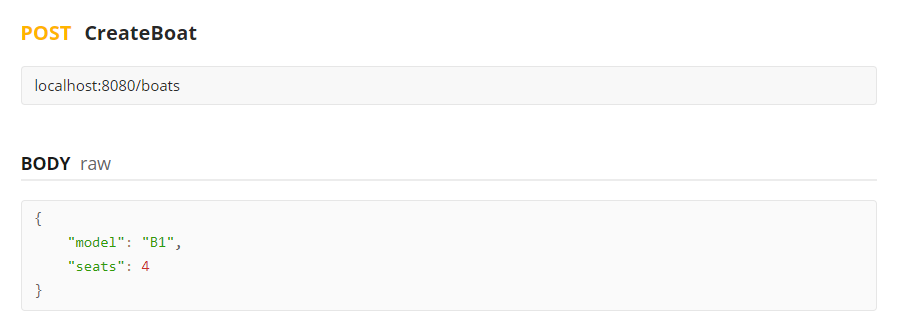
\includegraphics[width=\textwidth]{images/iterazione1/postman-api/CreateBoat.PNG}
    \centering
    \caption{API per la creazione di una barca}\label{creazione barca}
\end{figure}
\begin{figure}[htbp]
    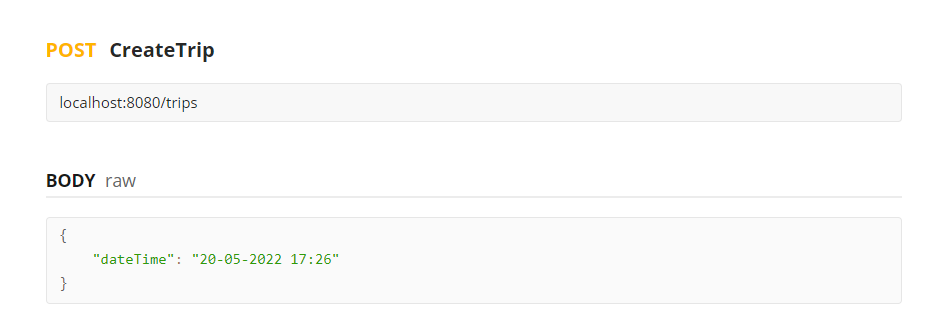
\includegraphics[width=\textwidth]{images/iterazione1/postman-api/CreateTrip.PNG}
    \centering
    \caption{API per la creazione di un'escursione}
    \label{creazione escursione}
\end{figure}
\begin{figure}[htbp]
    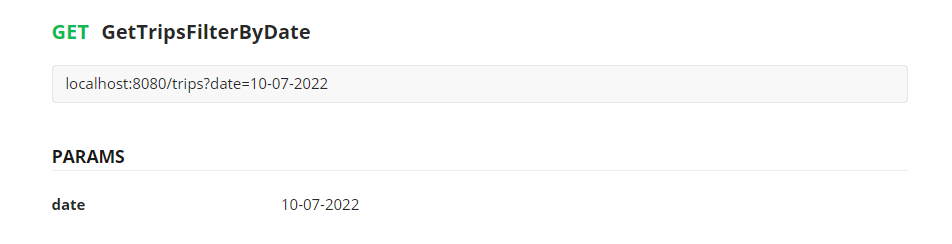
\includegraphics[width=\textwidth]{images/iterazione1/postman-api/GetTripFilterByDate.PNG}
    \centering
    \caption{API per la visualizzazione di escursioni relative ad un giorno specifico}
    \label{trip}
\end{figure}
\begin{figure}[htbp]
    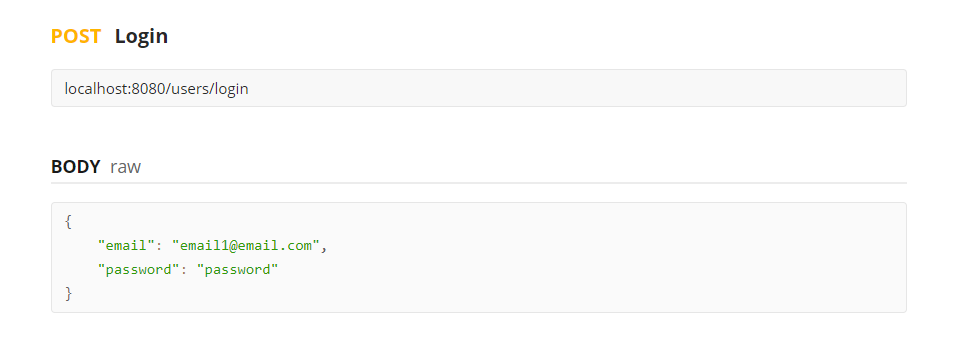
\includegraphics[width=\textwidth]{images/iterazione1/postman-api/Login.PNG}
    \centering
    \caption{API per il login di un utente}
    \label{login}
\end{figure}
\begin{figure}[htbp]
    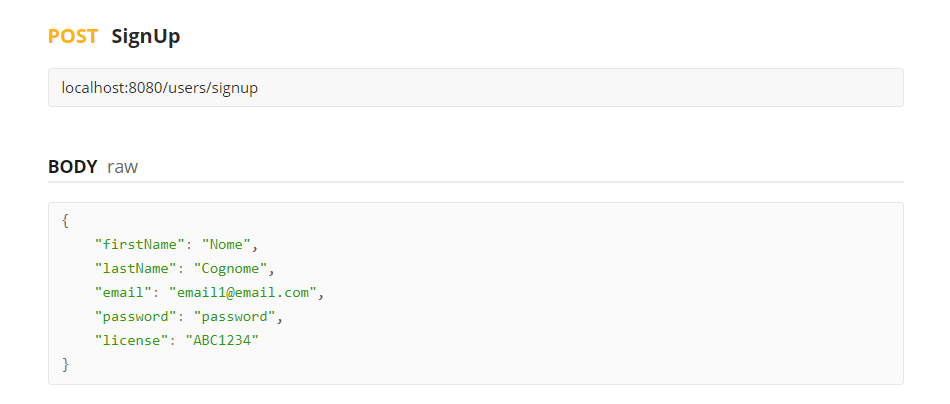
\includegraphics[width=\textwidth]{images/iterazione1/postman-api/SignUP.PNG}
    \centering
    \caption{API per la registrazione di un utente}
    \label{signup}
\end{figure}


\cleardoublepage 




